\subsection{Customer Choice Dynamics}
We first show that every customer exhibits the following behavior: until (s)he reaches the phase transition point $i_0(t)$, she visits $A$ only due to the exogeneity paramaeter, and after that (s)he always visits merchant $A$ till she receives the reward.
This behavior is cyclic, and repeats after every reward redemption.

\begin{lemma} $V(i)$ is an increasing function in $i$ if the following condition holds:
\begin{equation}
R > \frac{(1-\lambda)v}{1-\beta}
\end{equation}
And further, $V(i)$ can be evaluated as:
\begin{equation}
V(i) = \max\left\{ \frac{\lambda \beta V(i+1)+(1-\lambda)v}{1-(1-\lambda)\beta}, \beta V(i+1) \right\}
\end{equation}
\end{lemma}

\begin{proof}
First we show that $V(i)$ is an increasing function in $i$ by induction. We first show that if the condition above is satisfied, $V(k-1) < V(k) = R$. Suppose not, so $V(i) \geq R$. Then we have:
\begin{align*}
V(k-1) &= \lambda \beta V(k) + (1-\lambda)(v+\beta V(k-1)) \\
&= \frac{\lambda \beta R + (1-\lambda)v}{1-(1-\lambda)\beta} \\
&< \frac{\lambda \beta R + (1-\beta)R}{1-(1-\lambda)\beta} \\
&= \frac{R(1-(1-\lambda)\beta)}{1-(1-\lambda)\beta} = R
\end{align*}
But this is a contradiction, so $V(k-1) < V(k)$. Now assume $V(i+1) < V(i+2)$ for some $i < k-2$, we will show that this implies $V(i) < V(i+1)$. Suppose not, so $V(i) \geq V(i+1)$. As we did before we may upper bound $V(i)$.
\begin{align*}
V(i) &= \lambda \beta V(i+1) + (1-\lambda)(v+\beta V(i)) \\
&\leq (1-\lambda)v + \beta V(i) \\
\iff V(i) &\leq \frac{(1-\lambda)v}{1-\beta}
\end{align*}
But because $V(i+1) < V(i+2)$, we may lower bound $V(i+1)$.
\begin{align*}
V(i+1) &\geq \lambda \beta V(i+2) + (1-\lambda)(v+\beta V(i+1)) \\
&= (1-\lambda)v + (1-\lambda)\beta V(i+1) + \lambda \beta V(i+2) \\
&> (1-\lambda)+\beta V(i+1) \\
\iff V(i+1) &> \frac{(1-\lambda)v}{1-\beta}
\end{align*}
Again, we have a contradiction, so $V(i) < V(i+1)$, and $V(i)$ is an increasing function in $i$. Now we prove the second claim. We have the following:
\begin{align*}
V(i) &= \lambda \beta V(i+1) + (1-\lambda)\max\{v +\beta V(i), \beta V(i+1) \} \\
&= \max\{\lambda \beta V(i+1) + (1-\lambda)(v+\beta V(i)), \beta V(i+1) \}
\end{align*}

Assuming $V(i)$ is the left term in the above maximum, we may solve the equation for that term.
\begin{gather*}
V(i) = \lambda \beta V(i+1) + (1-\lambda)(v+\beta V(i)) \\
(1-(1-\lambda)\beta) V(i) = \lambda \beta V(i+1) + (1-\lambda)v \\
V(i) = \frac{\lambda \beta V(i+1) + (1-\lambda)v}{1-(1-\lambda)\beta}
\end{gather*}
And we get our claim.
\end{proof}

{\arpit Let's combine this theorem with the look-ahead parameter directly}

\begin{theorem} Assuming $V(i)$ is an increasing function in $i$, a phase transition occurs after the consumer makes $i_0$ visits to firm $A$, which evaluates to:
\begin{align*}
i_0 &= k - \left\lfloor \log_{\beta}\left(\frac{v}{R(1-\beta)}\right)\right\rfloor \\
&\equiv k-\Delta
\end{align*}
\end{theorem}

\begin{proof}
First we solve for the condition on $V(i+1)$ for us to choose firm $A$ over $B$ willingly.
\begin{gather*}
\beta V(i+1) > \frac{\lambda \beta V(i+1) + (1-\lambda)v}{1-(1-\lambda)\beta} \\
\iff \beta V(i+1) \left(1-\frac{\lambda}{1-(1-\lambda)\beta} \right) > \left(\frac{1-\lambda}{1-(1-\lambda)\beta} \right) v \\
\iff \beta V(i+1) \left(\frac{1-(1-\lambda)\beta -\lambda}{1-(1-\lambda)\beta} \right) > \left(\frac{1-\lambda}{1-(1-\lambda)\beta} \right) v \\
\iff \beta V(i+1) \left(\frac{(1-\lambda)(1-\beta)}{1-(1-\lambda)\beta} \right) > \left(\frac{1-\lambda}{1-(1-\lambda)\beta} \right) v \\
\iff \beta V(i+1) > \frac{v}{1-\beta} \\
\iff V(i+1) > \frac{v}{\beta(1-\beta)}
\end{gather*}
Let $i_0$ be the minimum state $i$ such that the above holds, so in particular $V(i_0) \le \frac{v}{\beta(1-\beta)}$ but $V(i_0+1) > \frac{v}{\beta(1-\beta)}$. We know because $V$ is increasing in $i$ (still need to prove), this point is indeed a phase transition: $V(i) > \frac{v}{\beta(1-\beta)}$ for all $i > i_0$, so after this point, the customer always chooses firm $A$. We may compute $V(i_0)$ easily using this fact.
\begin{equation*}
V(i_0) = \beta V(i_0+1) = \cdots = \beta^{k-i_0}V(k) = \beta^{k-i_0}R
\end{equation*}
Thus, we have the following:
\begin{gather*}
\beta^{k-i_0} \le \frac{v}{R\beta(1-\beta)} < \beta^{k-(i_0+1)} \\ 
\iff k-i_0 \ge \log_{\beta}\left(\frac{v}{R\beta(1-\beta)} \right) > k-(i_0+1) \\
\iff i_0 \le k - \log_{\beta}\left(\frac{v}{R(1-\beta)} \right) + 1 < i_0 + 1\\
\iff i_0 = k - \left\lfloor \log_{\beta}\left(\frac{v}{R(1-\beta)}\right) \right\rfloor \equiv k-\Delta
\end{gather*}
\end{proof}

With the inclusion of the look-ahead factor, the phase transition point depends on it, and we will refer to it as $i_0(t)$. Specifically, the dependence is as follows:

\begin{equation*}
  i_0(t)=\begin{cases}
    i_0, & \text{if $t \geq \Delta$}.\\
    k-t, & \text{otherwise}.
  \end{cases}
\end{equation*}

The above dependence reduces to the following after incorporating the look-ahead distribution:

\begin{equation*}
  i_0(t)=\begin{cases}
    i_0, & \text{wp } p,\\
    k, & \text{wp } 1-p.
  \end{cases}
\end{equation*}

{\arpit Discussion around what do the $i_0$ dependencies mean.}

{\arpit Discussion around setting $i_0 = 0$}

\subsection{Merchant Objective Dynamics}
We substitute the value of the phase transition point obtained above in the rate of revenue equations to reevaluate them. 
And since we assume that $\lambda$ and $t$ are drawn indepent of each other, we can separate the expectation terms and evaluate them sequentially, first over $t$, then over $\lambda$. This reduces the rate of revenues as follows:

\begin{align*}
RoR_A =& \underset{\lambda, t}E\left[\frac{k-R}{i_0(t)/\lambda + k - i_0(t)}\right]\\
                                       =& \underset{\lambda}E\left[p\cdot\frac{k-R}{i_0/\lambda + k - i_0} + (1-p)\frac{\lambda(k-R)}{k}\right]\\
                                       =& \underset{\lambda}E\left[p\cdot\frac{\lambda(k-R)}{k\lambda + i_0(1-\lambda)} + (1-p)\frac{\lambda(k-R)}{k}\right]\\
                                       =& p\cdot\frac{k-R}{(k-i_0)^2}\cdot\left(b(k-i_0) - i_0 \log\left(1 + \frac{b(k-i_0)}{i_0}\right)\right) + (1-p)\frac{b^2(k-R)}{2k}
\end{align*}

\begin{align*}
RoR_B =& \underset{\lambda, t}E\left[\frac{(i_0(t)\lambda - i_0(t))(1-v)}{i_0(t)/\lambda + k - i_0(t)}\right]\\
                                     =& \underset{\lambda}E\left[p\cdot\frac{(i_0/\lambda - i_0)(1-v)}{i_0/\lambda + k - i_0} + (1-p)\frac{(k/\lambda - k)(1-v)}{k/\lambda}\right]\\
                                     =& \underset{\lambda}E\left[p\cdot\frac{i_0(1-\lambda)(1-v)}{k\lambda + i_0(1-\lambda)} + (1-p)(1-\lambda)(1-v)\right]\\
                                     =& p\cdot\frac{i_0(1-v)}{(k-i_0)^2}\left(k\log\left(1+\frac{b(k-i_0)}{i_0}\right) - b(k-i_0)\right) + (1-p)(b-\frac{b^2}{2})(1-v)\\
\end{align*}

{\arpit
\begin{theorem}
When is $RoR_A > RoR_B$ at $i_0 = 0$?
\end{theorem}
}

At small values of $b$ the above evaluate to:
\begin{align*}
RoR_A =& p\cdot(k-R)\cdot\frac{b^2}{2i_0} + (1-p)\frac{b^2(k-R)}{2k}\\
                                       =& \frac{b^2(k-R)}{2}\left(\frac{p}{i_0} + \frac{1-p}{k}\right)
\end{align*}

\begin{align*}
RoR_B =& p\cdot\frac{i_0(1-v)}{(k-i_0)^2}\left(bk\frac{(k-i_0)^2}{i_0}- k\frac{b^2(k-i_0)^2}{2i_0^2} \right) + (1-p)(b-\frac{b^2}{2})(1-v)\\
                                     =& p\cdot(1-v)\left(bk- k\frac{b^2}{2i_0}\right) + (1-p)(b-\frac{b^2}{2})(1-v)\\
                                     =& b(1-v)\cdot \left(pk(1-\frac{b}{2i_0}) + (1-p)(1-\frac{b}{2})\right)
\end{align*}

{\arpit Talk about the framework in depth. That this can be used to find optimal $R$ and $k$. Also different distributions can be tested once the framework is ready}

\subsubsection{Proportional Promotion Budgeting}
First we look into the case when $A$ sets its reward value $R$ proportional to the product of the distance to the reward $k$ and the discount value $v$ provided by merchant $B$: \ie~ $R = \alpha k v$.
We refer to this case as proportional promotion budgeting.
Note $\alpha$ is a constant here.

\begin{theorem}
Under prportional promotion budgeting, the optimal reward distance that $A$ should set is $k = \frac{e}{\alpha(1-\beta)}$ at small values of $b$ and $k = \frac{e^{(1-\beta)t_1}}{\alpha(1-\beta)}$ for larger values.
\end{theorem}
\begin{proof}
{\arpit this proof needs to be rewritten, combined with the next section}
First merchant $A$'s objective evaluates to the following:
\begin{align*}
\underset{k}\max\{RoR_A\} \Leftrightarrow & \underset{k}\max\left\{\underset{\lambda}E\left[\frac{\lambda k}{k-\Delta(1-\lambda)}\right]\right\}\\
                          \Leftrightarrow & \underset{k}\max\left\{ \frac{1}{b}\int_{0}^{b} \frac{\lambda k}{k-\Delta(1-\lambda)}d\lambda \right\}\\
                          \Leftrightarrow & \underset{k}\max\left\{ \frac{k}{\Delta^2 b}\left(\Delta b - (k-\Delta)\log\left(\frac{k-\Delta(1-b)}{k-\Delta}\right)\right) \right\}\\
                          \Leftrightarrow & \underset{k} \max\left\{\frac{k}{\Delta}\left(1-\frac{k-\Delta}{b\Delta}\log\left(\frac{k-\Delta(1-b)}{k-\Delta}\right)\right)\right\}
\end{align*}
Now let $\theta = \frac{\Delta}{k}$. Then maximizing the above function is equivalent to maximizing the following function w.r.t. $\theta$ with keeping in mind the range that $\theta$ can follow.
\beq
\underset{k}\max\{RoR_A\} \Leftrightarrow \underset{\theta}\max\{f(\theta)\} \Leftrightarrow \underset{\theta}\max\left\{ \frac{1}{\theta} \left(1-\frac{1-\theta}{b\theta}\log\left(1 + \frac{b\theta}{1-\theta}\right)\right)\right\} 
\eeq
Let's look at the quantity $\frac{\Delta}{k}$.
\begin{align*}
\frac{\Delta}{k} = \frac{\log_\beta\left(\frac{1}{k(1-\beta)}\right)}{k} \sim \frac{\log(k(1-\beta))}{k(1-\beta)} 
\end{align*}
Now this value is maximized at $k = \frac{e}{1-\beta}$ and minimized at the maximum possible value of $k$ which is bounded above by $\frac{e^{(1-\beta)t_1}}{1-\beta}$ from the assumption of $t_1 \ge \Delta$.

When $b$ is small, the function $f(\theta)$ can be approximated by taking the second degree terms for the term inside the log. This gives:

\begin{align*}
f(\theta) \sim & \frac{1}{\theta} \left(1-\frac{1-\theta}{b\theta}\left(\frac{b\theta}{1-\theta} - \frac{\left(\frac{b\theta}{1-\theta}\right)^2}{2}\right)\right)\\
          = & \frac{b}{2(1-\theta)}
\end{align*}
Clearly $f(\theta)$ is maximized when $\theta$ is maximized. This happens as shown above at $k = \frac{e}{1-\beta}$

Whereas when $b$ is large, $f'(\theta)$ can be shown to be negative. Hence we get our result.

\end{proof}

Note that under equal-budgeting, we need $k > \frac{1-\lambda}{1-\beta}$ for $V$ to be increasing. We meet this condition when $k = \frac{e}{1-\beta} > \frac{1}{1-\beta} \geq \frac{1-\lambda}{1-\beta}$. Figure~\ref{fig:phase_trans} shows the percentage of visits needed for a ``forward-looking'' consumer to adopt the reward program as a function of $\beta$. (Here we should add our comments on cash back computations).

\begin{figure}[h!]
\begin{centering}
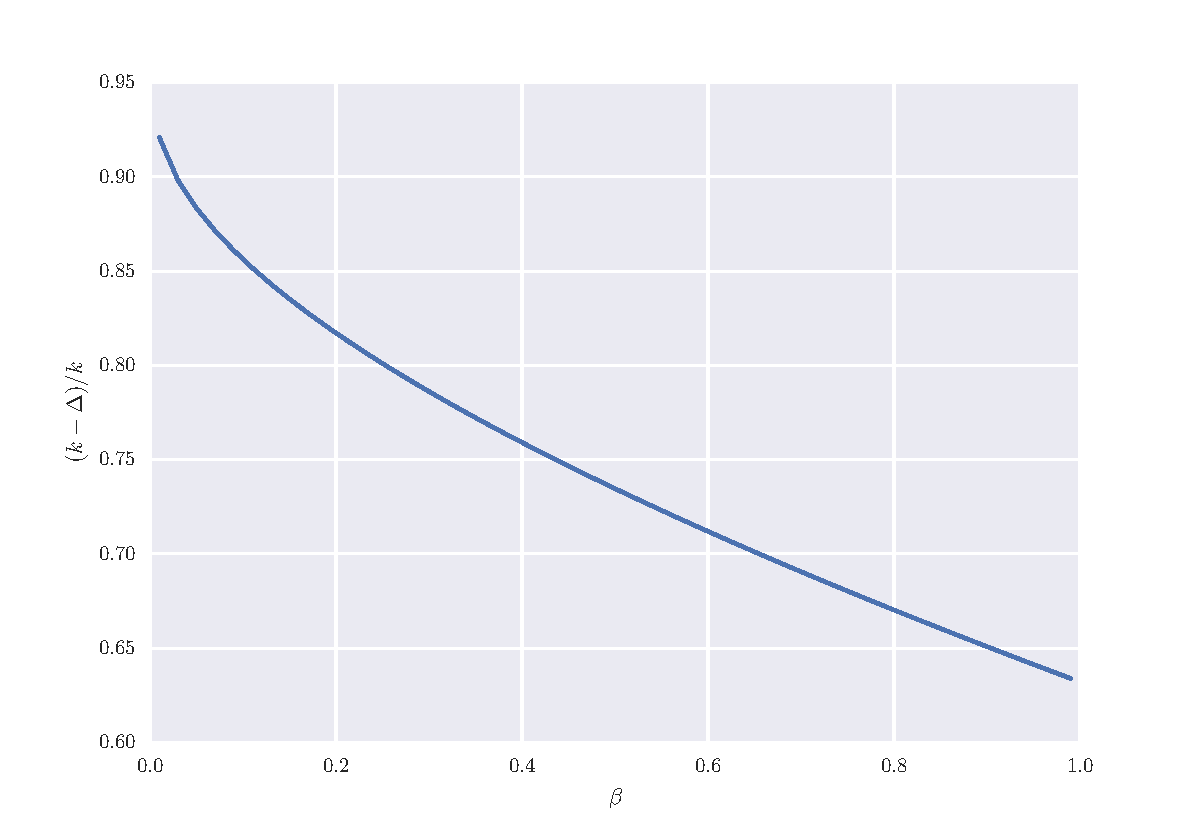
\includegraphics[scale = 0.75]{./figures/phase_trans.pdf}
\caption{We assume $k = e/(1-\beta)$ and equal-budgeting. The plot shows the percentage of extraneous visits needed for a ``forward-looking'' consumer needed to adopt the reward program as a function of $\beta$.}
\label{fig:phase_trans}
\end{centering}
\end{figure}

Now we consider the expected revenues of each firm under these conditions.

\beq
\underset{\lambda, t}E[RoR_A] = pk(1-v)\frac{1}{b}\int_0^b \frac{\lambda}{k-(1-\lambda)\Delta} \mbox{ } d\lambda + (1-p)(1-v)\frac{b}{2}
\eeq

\beq
\underset{\lambda, t}E[RoR_B] = pk(1-v)\frac{1}{b}\int_0^b \frac{1-\lambda}{k-(1-\lambda)\Delta} \mbox{ } d\lambda + (1-p)(1-v)\left(1-\frac{b}{2}\right)
\eeq

First notice that the ratio of expected revenues is independent of $v$, the price difference of the two firms. We observe this behavior in our simulations as well. Figure~\ref{fig:eq_budg_vary_v} shows the revenue rates of $A$ and $B$ as a function of $b$ for different values of $v$. We see that the relative rates do not vary with $v$; changing $v$ only changes the absolute revenue rates of each firm, putting more money into the rewards given out. We see that $b$ must be pretty large for firm $A$ to make more money than firm $B$. 

\begin{figure}[h!]
\begin{centering}
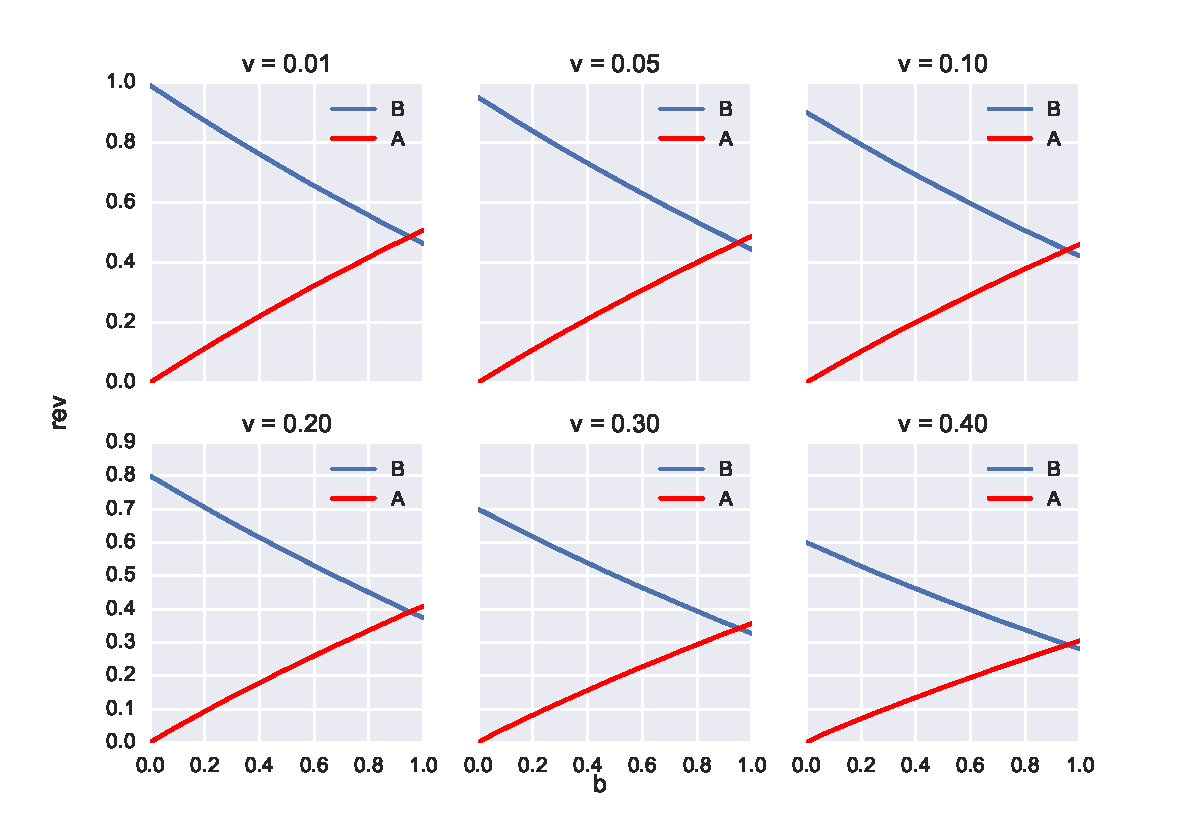
\includegraphics[scale = 0.75]{./figures/eq_budg_vary_v_p05.pdf}
\caption{Rates of revenue for $A$ and $B$ with equal-budgeting as a function of $b$ for various $v$. Fixed $p = 0.5$, $\beta = 0.9$ and $k = e/(1-\beta)$.}
\label{fig:eq_budg_vary_v}
\end{centering}
\end{figure}

[Not sure if we should include] We may solve for the $b$ such that the expected revenues are equal, which occurs if when the following holds (excluding work for now).
\begin{equation*}
b-\frac{2k(k-\Delta)p}{(1-p)b\Delta^2}\log \left(\frac{k-(1-b)\Delta}{k-\Delta} \right) = 1-\frac{p}{1-p} \frac{2k-\Delta}{\Delta}
\end{equation*}

Note from the above that $p$, the probability of a consumer being ``forward-looking'' does affect the ratio of expected rates of revenue. Figure~\ref{fig:eq_budg_vary_p} shows simulation results for the rates of revenue of $A$ and $B$ for various values of $p$ with everything else fixed. We see that as $p$ increases, the $b$ required for the reward program to become more profitable than not using one decreases.

\begin{figure}[h!]
\begin{centering}
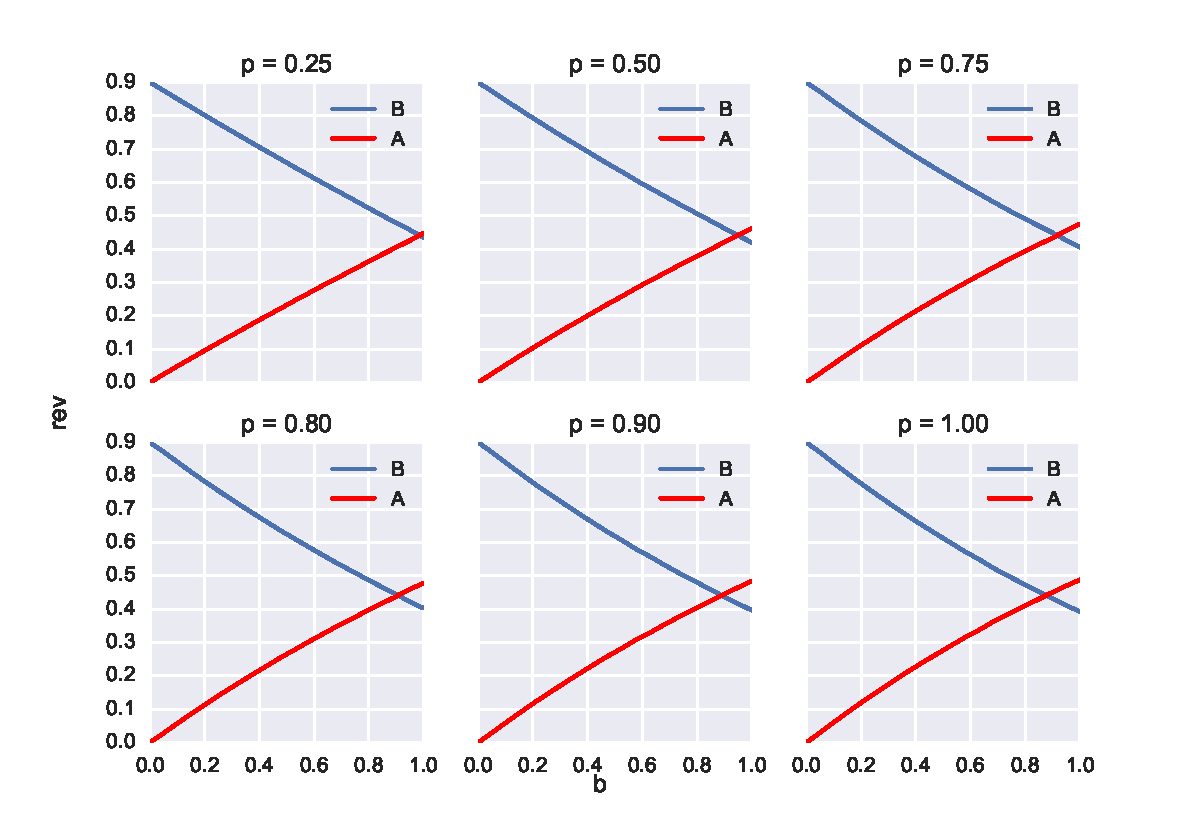
\includegraphics[scale = 0.75]{./figures/eq_budg_vary_p_v01.pdf}
\caption{Rates of revenue for $A$ and $B$ with equal-budgeting as a function of $b$ for various $p$. Fixed $v = 0.1$, $\beta = 0.9$ and $k = e/(1-\beta)$.}
\label{fig:eq_budg_vary_p}
\end{centering}
\end{figure}

\subsubsection{Non Strategic Merchant $B$, and Unequal Promotion Budgeting}

Now we consider scenarios in which firms $A$ and $B$ have different budgets. First we consider the case where the budgets are still proportional, i.e. $R = \alpha \cdot kv$ for some fixed $\alpha$. Now the expected rate of revenue of $A$ is given by the following, while that of firm $B$ is unchanged. Therefore the ratio of expected revenue rates may now depend on $v$.
\beq
\underset{\lambda, t}E[RoR_A] = pk(1-\alpha v)\frac{1}{b}\int_0^b \frac{\lambda}{k-(1-\lambda)\Delta} \mbox{ } d\lambda + (1-p)(1-\alpha v)\frac{b}{2}
\eeq

Following the same logic of Theorem 3.2, the expected revenue rate of $A$ is maximized at $k = \frac{e}{\alpha(1-\beta)}$ at small values of $b$ (need to do again for larger values). For this value of $k$, $\Delta$ is fixed for all $\alpha$ ($\Delta = \left \lfloor \log_{\beta} \left(\frac{1}{e} \right) \right \rfloor$), so we must have $\alpha \leq \frac{e}{\Delta(1-\beta)}$ for $k \geq \Delta$ to hold. When $\beta = 0.9$, this upperbound on $\alpha$ is about 3.


\begin{theorem}
Suppose firm $A$ fixes its price at 1, and firm $B$ chooses a price of $1-v$. Given a consumer distribution defined by $p$ - with probability $p$, a consumer is fully forward looking and probability $1-p$ the customer does not look ahead at all - $b$ - each consumer's monopoly factor to firm $A$ is drawn as $\lambda~\sim Unif(0,b)$ and $\beta$ - the customer's discout factor. Then firm $A$ may choose to give a reward of $\alpha v < 1$ to customers after $k$ visits. It should run a reward program if the following condition holds.
\begin{equation}
\frac{1}{b}\left(1-\frac{e-1}{b}\log \left(1+\frac{b}{e-1} \right) \right) \geq \frac{1-(1-p)(1-\alpha v)}{2pe(1-\alpha v)}
\end{equation}
Define the function on the left-hand side above as $g(b)$.
\end{theorem}

\begin{proof}
Firm $A$ always sells the good for price 1. If it chooses to run a reward program its expected rate of revenue is given by:
\begin{equation*}
\underset{\lambda, t}E[RoR_A] = pk(1-\alpha v)\frac{1}{b}\int_0^b \frac{\lambda}{k-(1-\lambda)\Delta} \mbox{ } d\lambda + (1-p)(1-\alpha v)\frac{b}{2}
\end{equation*}
If it does not run a reward program, then the only visits it will receive are exogenous visits. In this case, its expected rate of revenue is simply $\frac{b}{2}$. We consider a reward program to be profitable if its expected rate of revenue is at least that of the non-reward program expected revenue rate.
\begin{gather*}
pk(1-\alpha v)\frac{1}{b}\int_0^b \frac{\lambda}{k-(1-\lambda)\Delta} \mbox{ } d\lambda + (1-p)(1-\alpha v)\frac{b}{2} \geq \frac{b}{2} \\
\iff \frac{pk(1-\alpha v)}{\Delta}\left(1-\frac{k-\Delta}{b\Delta}\log \left(\frac{k-(1-b)\Delta}{k-\Delta} \right) \right) \geq \frac{b}{2}(1-(1-p)(1-\alpha v)) \\
\iff pe(1-\alpha v)\left(1-\frac{e-1}{b}\log \left(1+\frac{b}{e-1} \right) \right) \geq \frac{b}{2}(1-(1-p)(1-\alpha v)) \\
\iff \frac{1}{b}\left(1-\frac{e-1}{b}\log \left(1+\frac{b}{e-1} \right) \right) \geq \frac{1-(1-p)(1-\alpha v)}{2pe(1-\alpha v)}
\end{gather*}
Where we have used the work from Theorem 3.2 as well as the fact that the optimal $k$ is given by $\frac{e}{\alpha(1-\beta)}$, making $\Delta \approx \frac{1}{1-\beta}$. 
\end{proof}

Note that the above condition on $b$ is rather complicated, so we have plotted it as a function of $b$ below. First we notice that $g(b)$ is decreasing in $b$. So for a fixed evaluation of $x \equiv \frac{1-(1-p)(1-\alpha v)}{2pe(1-\alpha v)}$, we are in one of the following cases:
\begin{enumerate}
\item
$x \geq g(0)$. So no value of $b$ makes the reward program profitable.
\item
$x \leq g(1)$. So any value of $b$ makes the reward program profitable.
\item
$x = g(b_0)$ for some $b_0 \in (0,1)$. So the reward program is profitable for all $b \leq b_0$ and not otherwise.
\end{enumerate}

\begin{figure}[h!]
\begin{centering}
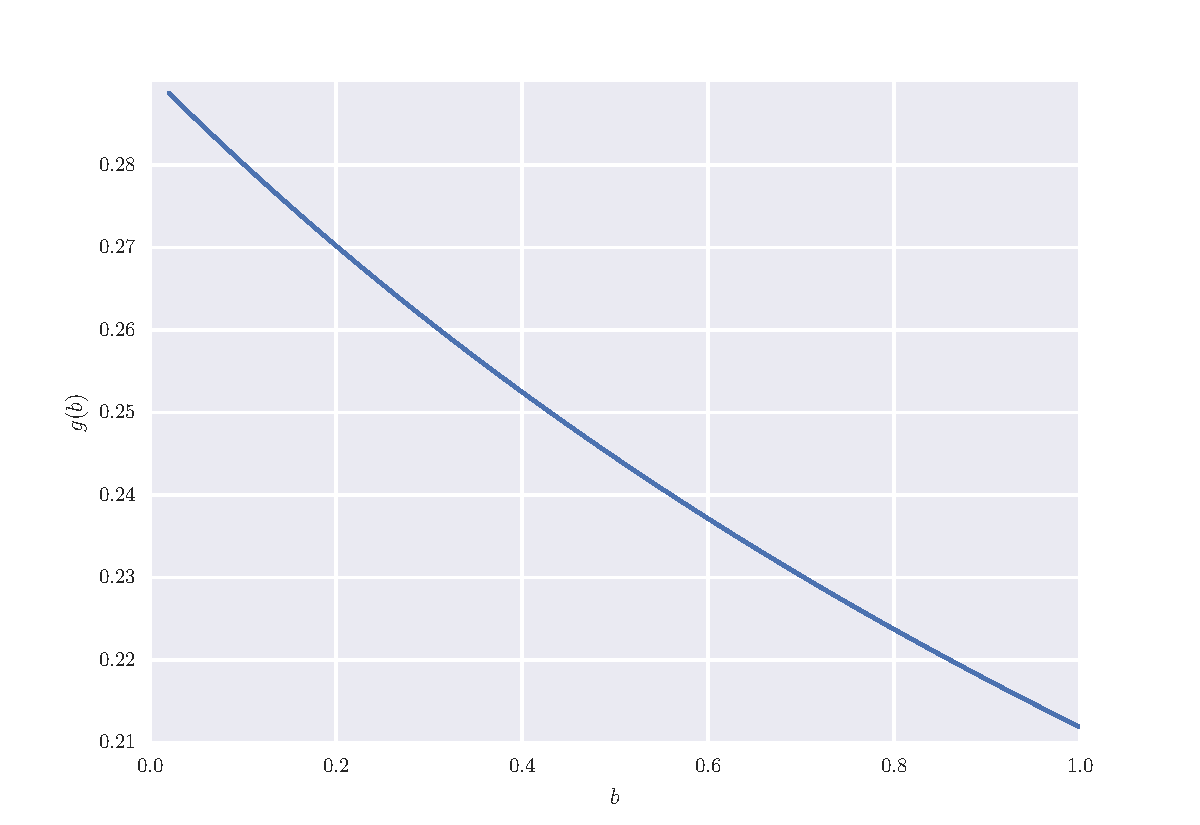
\includegraphics[scale = 0.75]{./figures/b_plot.pdf}
\caption{Function governing profitability of reward program for firm $A$ as a function of $b$.}
\label{fig:b_plot}
\end{centering}
\end{figure}

Now we can take a look at the right hand side of the profitability condition. Let $h(p, \alpha, v) = \frac{1-(1-p)(1-\alpha v)}{2pe(1-\alpha v)}$. It is easy to see that for all values of $p$, $\alpha$ and $v$, $\frac{\partial h}{\partial p} < 0$, $\frac{\partial h}{\partial v} > 0$ and $\frac{\partial h}{\partial \alpha} > 0$. These partial derivative signs mean that as $p$ increases (fixing $v$ and $\alpha$), the interval of profitable $b$'s can only increase. This result make sense intuitively - as the $p$ increases, the number of consumers looking ahead does as well, so more people adopt the reward program. However, increasing either $\alpha$ or $v$ (keeping others fixed), the interval of profitable $b$'s can only decrease. Thus, increasing the reward while keeping $p$ fixed means that in order for the reward program to remain profitable, the profits earned without the reward program must simultaneously decrease, which occurs with decreasing $b$.
